% Capítulo 2 - Contextualização ou definição do problema

\chapter{Fundamentação teórica}
\simb[$ f_0 $ (frequência fundamental da fala)]

\section{Prosódia}
\citeonline{tts-book,ladd} descrevem como parâmetros principais da prosódia o
\emph{pitch} -- termo intercambiável com frequência fundamental ou $f_0$ --,
intensidade e duração. Outros nomes para os mesmos fenômenos também são
utilizados: \citeonline{moraes1998}, por exemplo, separa as características
principais da prosódia em \emph{stress}, \emph{accent} e \emph{rhythm}. O que as
definições têm em comum, porém, é que a prosódia compreende melodia e ritmo da
fala, permitindo expressão comunicativa e realização de fenômenos
``sintáticos'', como a acentuação de sílabas tônicas. Como os elementos
prosódicos estão alinhados, isto é, ocorrem paralelamente a segmentos como
sílabas e fones, a prosódia é dita um fenômeno suprassegmental \cite{ladd}.

Além desses componentes principais, \citeonline{taylor2009}
destaca como aspecto relevante para análise entoacional o \emph{downdrift}
(declinação), isto é, a queda gradual do valor de $ f_0 $ durante uma enunciação.

% melhor: ladd, $ f_0 $, intensidade e duração! p.10 lucente

\subsection{Função prosódica}
\citeonline{taylor2009} argumenta que uma das dificuldades do desenvolvimento de
um bom modelo de prosódia se deve à falta de consideração da função comunicativa
da fala, isto é, comumente análises são feitas ignorando o contexto da intenção
do locutor. Apresenta, então, as três principais funções comunicativas para
prosódia, descritas a seguir.

% n general, affective prosody has a fairly direct meaning-to-form relationship and hence the more extreme the form the more extreme the emotion. This implies that, unlike verbal language, the affective prosody system is not arbitrary with regard to meaning/form. A number of emotion categorisation systems have been proposed. One common theory holds that there are six basic emotions (anger, happiness, sadness, disgust, fear and surprise) from which follow a number of secondary emotions such as puzzlement or intrigue [110], [113], [153]. Some however argue that there is no fixed set of emotions and rather emotion is best expressed in a multi-dimensional system. One such proposal advocates three independent axes of emotion called activation, evalu- ation and power [393], [126].
% In addition to emotion, affective prosody includes speaker attitude. The difference between emotion and attitude is that only emotion can exist independent of communication. As an illustra- tion; you can be happy on your own, but you need someone else to be sarcastic with. Apart from this distinction, attitude functions similarly to emotion in that it is fairly direct, has a significant degree of universality and does not have a arbitrary or dual nature.
\paragraph{Afetiva} A prosódia afetiva é utilizada para demonstrar emoções,
atitude e intenção do locutor, e está praticamente ausente da forma escrita.
Mesmo para diferentes línguas, os contornos melódicos associados a diferentes
emoções são semelhantes, de forma que conseguimos deduzir relativamente bem uma
intenção ou emoção de um locutor que fala uma língua estrangeira mesmo sem
compreender o significado de cada palavra individualmente.

\paragraph{Suprassegmental} Quando uma mensagem é dita de maneira declarativa,
sem conteúdo afetivo significativo -- descrita como \emph{discourse neutral} --,
ainda é possível observar variação de \emph{pitch}, intensidade e duração. Na
abordagem de \citeonline{taylor2009}, essa parte da prosódia, dita
suprassegmental, não é considerada conteúdo prosódico verdadeiro, mas sim um
aspecto da fonética verbal. É possível ainda pensar em prosódia ``real'', ou
seja, afetiva e aumentativa, como desvios dos parâmetros suprassegmentais.

% If a sentence is spoke with little or no affective content, ie. in a discourse neutral manner, we still see characteristic patterns in the phrasing, rhythm, pitch, voice quality and timing. Typical effects include phones at the ends of sentences or phrases being lengthened, syntactically salient words (e.g. heads) having more emphasis, $ f_0 $ levels being higher at the starts of sentences and so on.
\paragraph{Aumentativa} Além da prosódia afetiva, é possível desviar da prosódia
padrão para assegurar a comunicação efetiva de uma mensagem sem adicionar
informação ao conteúdo que está sendo dito. É usada, por exemplo, para
enfatizar palavras, desambiguando uma mensagem que poderia ser interpretada de
diferentes formas.

\section{Sistemas \emph{text-to-speech}}
\citeonline{ssml} definem \emph{text-to-speech} como ``o processo de geração
automática de fala a partir de texto ou texto anotado'' (tradução nossa). São
utilizados em leitores digitais, assistentes pessoais para \emph{smartphones},
aprendizagem de linguagens, entre outros.

Sistemas TTS são compostos por múltiplos subsistemas. Como veremos na seção
\ref{sistemas}, algumas implementações de TTS são modulares, permitindo
desenvolvimento paralelo de cada componente individual. Isso possibilita que
pesquisas possam focar em melhorias de uma parte específica do sistema sem
necessidade de entendimento total. Neste trabalho, por exemplo, estudamos
especificamente o módulo de prosódia.

\subsection{Estrutura}
Na literatura, cada sistema TTS normalmente emprega algoritmos diferentes,
resultando em múltiplas arquiteturas possíveis para conversão de texto em fala.
Apesar disso, \citeonline{tts-book} propõe uma arquitetura geral, dividindo os
sistemas em duas partes principais descritas na Figura \ref{fig:tts-arch}.

\begin{figure}[!htbp]
\centering
\scalebox{0.80}{
    \begin{tikzpicture}[auto, >={Latex[inset=0pt, length=3mm, angle'=28,round]}, box/.style={draw,rounded corners,text width=4.5cm,align=center}]
    \node[] (txt) {Texto};
    \node[box, right=of txt] (nlp)
        {Processamento de linguagem natural};
    \node[box, right=of nlp] (dsp)
        {Processamento digital de sinais};
    \node[right=of dsp] (fal)
        {Fala};

        \node[box, fit=(nlp)(dsp), label=Sistema \emph{text-to-speech}] (tts) {};

    \draw[->] (txt) -- (nlp);
    \draw[->] (nlp) -- (dsp);
    \draw[->] (dsp) -- (fal);
    \end{tikzpicture}
}
\caption[Arquitetura geral de sistemas TTS]{Arquitetura geral de sistemas TTS. Fonte: Adaptado de \citeonline{tts-book}}
\label{fig:tts-arch}
\end{figure}

É comum encontrar em outros trabalhos o termo \emph{front end} para o
bloco de processamento de linguagem natural e \emph{back end} para o bloco de
processamento digital de sinais. Doravante utilizaremos essa nomenclatura.

\subsection{\emph{Front end}}
O \emph{front end} de um sistema TTS é responsável pela conversão do texto em
sua representação em fones juntamente com parâmetros prosódicos. Em outras
palavras, o bloco é responsável por determinar a pronúncia de cada palavra do
texto, incluindo o contorno melódico e ritmo da fala. As definições seguintes
são adaptadas de \citeonline{martinjurafsky}.

\subsubsection{Normalização de texto}
O processo de conversão de texto para fala começa com o processamento do texto a
fim de gerar uma representação grafêmica. A primeira etapa da normalização é a
separação de sentenças, isto é, devem ser encontrados os limites de cada frase
do texto. Frases que terminam com siglas ou abreviações podem dificultar o
processo, como pode ser observado no exemplo seguinte.

Posteriormente, devem-se transformar símbolos, abreviações, siglas e outras
\emph{non-standard words} em suas representações pronunciáveis. Como exemplo,
``V. Exa. me deve R\$ 50'' deve ser lido como ``vossa excelência me deve
cinquenta reais''.

Por último, deve ser realizada a desambiguação de homônimos heterófonos: em
``Gosto de pão'', ``gosto'' pode ser pronunciada como ``gôsto'' ou ``gósto'',
por exemplo.

\subsubsection{Conversão grafema-fone}
Com o texto normalizado, é preciso converter as letras em uma representação
pronunciável, ou seja, fonemas ou fones. Para isso, normalmente é composto um
conjunto de regras \emph{letter-to-sound} ou letra-som, contendo as pronúncias
comuns para sequências de letras, juntamente a um dicionário de pronúncia com
palavras que não se adequam às regras. Para cada palavra, é feita uma busca no
dicionário, e caso não seja encontrada, utilizam-se as regras.

% TODO: letra vs. grafema

% Palavras não-padrão são colocadas num dicionário de pronúncia. O resto é
% calculado de acordo com regras letra-som.
% Context-dependent e independent. Abordagens por machine learning ou regras.
% A conversão grafema-fone (ou fonema) consiste em transformar o texto normalizado
% em fones, ou seja, uma sequência de caracteres em uma sequência de fones.

\subsubsection{Geração de prosódia}
\label{gerpros}
A partir do texto e fones gerados nas etapas anteriores, deve-se estimar
\emph{pitch}, intensidade e duração. \citeonline {taylor2009} explica que o
desafio para implementação deste componente é que o texto praticamente não
possui informação prosódica. \citeonline{tts-book} divide as abordagens para
geração de prosódia automática em três técnicas: heurísticas derivadas a mão,
sistemas baseados análise gramátical e métodos baseados em corpus.

Destacamos na seção \ref{prosafe} uma quarta abordagem possível, que consiste na
anotação automática ou manual de prosódia, ênfase ou emoção, fornecendo
``dicas'' a sistemas TTS para melhor geração de prosódia.

% \subsection{Prosódia como elemento extra-textual}
% \citeonline{taylor2009} argumenta que a geração de prosódia afetiva é árdua e
% depende de uma compreensão do texto. Ainda fala que, até a data de publicação do
% livro, nenhuma solução satisfatória foi encontrada e os sistemas TTS atuais
% pecam nesse aspecto.
% Considerando o texto como sequência de palavras, é difícil determinar prosódia
% afetiva.
% Gerar a prosódia certa é uma questão de Natural Language Understanding, isto é,
% é preciso entender o texto para gerar os contornos melódicos afetivos.
% From this we can conclude that in situations where the text genre is quite factual, it is usually sufficient to generate speech from the verbal message only, and so all that is required is the gen- eration of the suprasegmental part of the signal; the affective part of prosody is ignored. In other text genres the situation is significantly more difficult, and if say a dialogue from a play is read in this fashion (or more likely) responses from a computer dialogue system, the generated speech can sound somewhat dull and removed. Finally, we see that mimicking a genuinely good human reader is very difficult indeed, as they will be performing an actual comprehension of the text, and then generating their own prosody. In no way are they simply decoding the prosody from the text and then speaking it aloud, as they can do with the words. To date, no satisfactory solution has been found to this problem, and so current text-to-speech systems are, unfortunately, lacking in this regard.

% \subsection{Contornos melódicos}
% \citeonline{moraes2008} analisa para a mesma frase ``Renata jogava'' utilizando
% o modelo ToBI uma mesma frase falada com intenções diferentes analisando como a
% entoação afeta a intenção percebida.


% In text-to-speech, our interest is of course to generate prosody from text. This is problematic in that text mostly encodes the verbal component of language; prosody is by and large ignored. Given that prosody is such a vital part of spoken language, how then is it possible that written communication can even work

% decide to use neutral prosody, and the suprasegmental effects that need to be
% synthesised can be found from the verbal part of the message. For more emotive
% messages, or in cases where we think we need significant use of augmentative
% prosody, we have a fairly serious problem. This is because we have no means of
% knowing what prosody the speech should be encoded with; the message that we
% found from the text has no explicit clues as to what the prosody should be.
% (taylor p 37)
%  I wanted to go to London, but could only get tickets for France there seems to be two main intonation phrases, their boundary occurring at the comma
%  there is often a slight drop in $ f_0 $ from the beginning of an intonation phrase to its end, which resets at the beginning of a new intonation phrase
% A very high-precision rule is the one we saw for sentence segmentation: insert a boundary after punctuation. Another commonly used rule inserts a phrase boundary before a function word following a content word.

\subsection{\emph{Back end}}
\label{backend}
% martin jurasfky p275
Com o texto de entrada transformado em fones e informação prosódica, um
\emph{back end} é responsável por gerar uma forma de onda, ou seja, o áudio a
ser reproduzido pelos alto-falantes. \citeonline{martinjurafsky,taylor2009} separam
algoritmos de síntese em três classes, listadas a seguir.

\subsubsection{Síntese articulatória}
Sintetizadores articulatórios sintetizam fala através de modelos matemáticos,
aproximando o aparelho fonador por uma série de tubos abertos. Pequenas
alterações nos parâmetros de entrada podem gerar uma grande variação de sons. Em
contrapartida, é difícil encontrar uma correspondência entre o texto de entrada
e os parâmetros necessários para o sintetizador.

\subsubsection{Síntese por formantes}
\label{formant}
Na Figura \ref{fig:spectrum}, podem-se ver duas representações para uma gravação de
fala. Acima tem-se a amplitude em função do tempo e abaixo, frequências em
função do tempo, isto é, a decomposição espectral. O conteúdo frequencial é
majoritariamente composto por múltiplas senoides -- também ditas harmônicas --
de frequências $ f_0 $, $ f_1 = f_0 * 2 $, $ f_2 = f_0 * 3 $ e $ f_3 = f_0 * 4
$. A frequência mais baixa é dita frequência fundamental ou apenas $ f_0 $,
emitida pela glote. As três senoides imediatamente acima, f1, f2 e f3, são
chamadas formantes, geradas pela ressonância do filtro resultante da posição da
língua, queixo e lábio, alterando a intensidade de cada componente frequencial.
A variação de intensidade de cada formante determina a vogal percebida.
Sintetizadores por formantes são tentativas de modelagem da fala humana pela
geração computacional dessas ondas. Apesar da simplicidade do modelo, além das
senoides principais, pode ser visto na Figura \ref{fig:spectrum} conteúdo
harmônico significante no sinal de uma fala humana.  Ao ignorar-se essa parte,
dita residual, a fala sintetizada é perceptivelmente robótica.

\begin{figure}
  \centering
    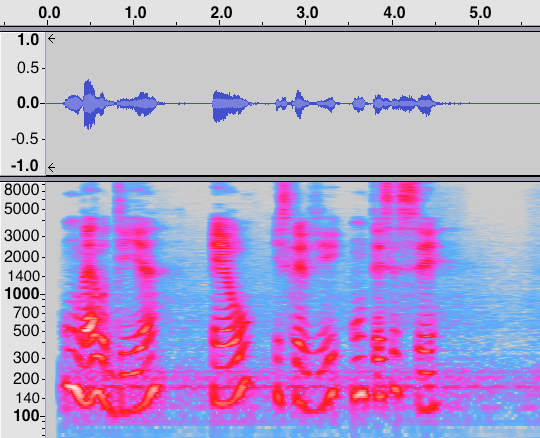
\includegraphics[width=0.5\textwidth]{Imagens/espectro.png}
  \caption[Representações temporal e espectral de uma gravação de voz]{Representações temporal (acima) e espectral (abaixo) de uma gravação de voz. Fonte: própria}
  \label{fig:spectrum}
\end{figure}

% quanto a $ f_0 $, f1, ver Taylor p. 185/161

\subsubsection{Síntese concatenativa}
Devido aos problemas destacados para as outras duas abordagens, a maior parte
dos sistemas TTS, até alguns anos atrás, utilizava síntese concatenativa, que
consiste na gravação de múltiplas frases posteriormente divididas
em fragmentos de granularidade variável, como ilustrado a seguir.

Para vocabulários com poucas palavras, como um sistema de anúncios de um metrô, é
suficiente gravar frases completas e palavras que podem variar dentro da frase.
Ao enunciar ``Este metrô para nas estações Catete, Glória, Cinelândia [...]'',
por exemplo, o fragmento ``Este metrô para nas estações'' pode advir de uma
única gravação, enquanto os nomes individuais das estações são provenientes de
outras gravações, concatenadas. Para obter sistemas TTS mais flexíveis, porém,
as gravações devem ser separadas em unidades menores, como fones ou dífonos --
 pares de fones -- que podem ser então concatenados para formar até mesmo
palavras que não foram gravadas.

Mais recentemente, foi popularizada uma nova classe de algoritmos para
síntese concatenativa denominada \emph{unit selection synthesis}, abordagem
probabilística que funciona através da minimização de duas função de custo, uma
para fones individuais e outra para a junção entre dois fones.
\citeonline{black} argumenta que, com advento desse tipo de síntese, a fala
gerada passou a ser natural o suficiente para ser possivelmente confundida com a de um humano.

\subsection{Síntese por \emph{Hidden Markov Models} e \emph{Deep Neural Networks}}
\label{hmmsynthesis}
\citeonline{zen} descrevem síntese por \emph{Hidden Markov Models} como uma
maneira paramétrica de produzir fala. Nela, um banco de dados com gravações é
utilizado para treinar um modelo a partir de múltiplos parâmetros de entrada
dividos em duas categorias: \emph{excitation parameters} e
\emph{spectral parameters}. Com este método de síntese de fala, há unificação
dos módulos de \emph{front end} e \emph{back end}. Mais recentemente, esse
modelo, denominado \emph{Statistical Parametric Speech Synthesis} foi adaptado
para utilizar redes neurais profundas no lugar de cadeias de Markov
\cite{dnngoogle}. Os resultados mais naturais para síntese de fala até o momento
foram obtidos por este paradigma.

% However, by properly combining these two, we may be able to obtain a first-rate complementary hybrid approach that can solve their respective drawbacks while retaining all their advantages. In the near fu- ture, we may find the holy grail of corpus-based speech synthe- sis fusing statistical parametric and unit-selection synthesi

% Statistical parametric speech synthesis provides a new frame- work for jointly optimizing the front-end (text analysis) and back-end (waveform generation) modules of text-to-speech (TTS) systems. These two modules are conventionally con- structed independently. The text-analysis module is trained us- ing text corpora and often includes statistical models to analyze text, e.g., the phrasing boundary, accent, and POS. The wave- form generation module, on the other hand, is trained using a labeled speech database. In statistical parametric synthesis, this module includes acoustic models. If these two modules are jointly estimated as a unified statistical model, it is expected to improve the overall performance of a TTS system. Based on this idea, Oura et al. proposed an integrated model for linguistic and acoustic modeling and demonstrated its effectiveness (Oura et al., 2008a).
% 
% \subsubsection{Síntese por \emph{Deep Neural Networks}}

% Intonational phrase: sintagmas entoacionais
% Tone boundary: fronteira prosódica?
% Pitch accent: acento de pitch

% https://www.ime.usp.br/~cpaz/downloads/algorithm-portuguese.pdf

% http://hts.sp.nitech.ac.jp/
% Algumas vozes para o MaryTTS \cite{marytts} utilizam HMMs, isto é, Modelos
% ocultos de Markov para \emph{unit selection}. Há, inclusive, uma voz brasileira
% feita a partir de HMMs: \cite{couto}.
% Projetos mais recentes como \cite{merlin,dnngoogle} utilizam redes neurais para
% estimação de parâmetros. O trabalho da Google informa? que a estimação da curva
% $ f_0 $ é uma possível melhoria.
